\section{Results}

The results section is split into three components: model selection, estimation, and estimation validation. In the section model selection we demonstrate that the neural mass model can mimic numerous dynamics observed in hippocampal EEG. For the estimation results we show that the unscented Kalman filter can be used to estimate the synaptic gains and input mean of a neural mass model with EEG observations. In estimation validation we then explore how descriptive the model estimates are of the recorded EEG. This is achieved by simulating data using the estimated synaptic gains and input mean. The simulated data is then compared to the recorded EEG in order to determine whether the estimates are capable of replicating the key characteristics observed.

\subsection{Model Selection}

The neural mass model of the hippocampus has been shown to be capable of replicating the frequency dynamics of hippocampal EEG~\citep{wendling2002epileptic}. In Figure~\ref{fig: EEG} two EEG traces are demonstrated, the first of recorded EEG from an animal that has had tetanus toxin injected into its hippocampus, and the second of simulated data using the neural mass model. The simulated data is generated by altering the synaptic gains and the input mean of the neural mass model of the hippocampus. In both traces the red dashed lines indicate the beginning and end of a seizure. Their is a clear relationship between the amplitude of the simulated data and the recorded EEG. In particular, at seizure onset both amplitudes of the simulated and recorded data increase. Prior to seizure termination their is a marked decrease in amplitude in both the recorded and simulated data. 
Even though their are clear similarities between the two traces, their are also clear differences. These differences are due to the input to the neural mass model, which is stochastic. Since the input is stochastic for the model, and unknown for the recorded EEG their will always be differences between the two. However, using this technique we can capture the dynamics that are important in terms of seizure initiation and termination. In this study, we evaluate what are the most likely set of physiological parameters that describe the transitions between seizure and non-seizure, and how these parameters alter during seizure.

\begin{figure}[ht]
 	\centering
 		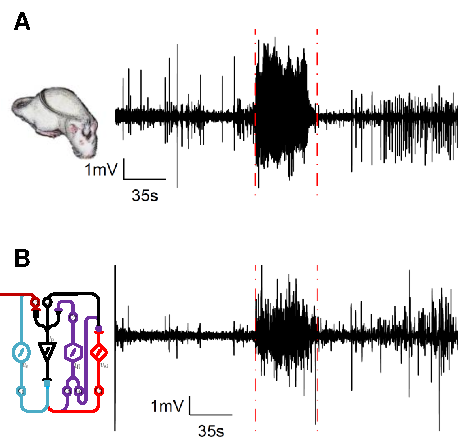
\includegraphics{fig/EEG.pdf}
 	\caption{Recorded and Simulated EEG. (\textbf{A}) Recorded EEG from an animal that has had a hippocampal tetanus toxin injection. (\textbf{B}) Simulated data generated from the neural mass model of the hippocampus. The red dotted lines indicate the start and end of a seizure in both traces.}
 	\label{fig: EEG}
 \end{figure}

\subsection{Estimation}

Hippocampal EEG can be mimicked by altering the synaptic gains of the neural mass model. However, a recent study has shown that there are network changes involved in seizure initiation and termination~\citep{truccolo2011single}. Therefore, we also consider the input mean to the modeled neural mass to be time varying. For this study, we have used recordings from four different control animals, and consider four seizures from each of them. All parameters are initialised identically and the same algorithm is used for all recordings. 

The first of five traces in figures \textbf{A}-\textbf{D} show the recorded EEG of seizure one for each animal~(Figure~\ref{fig: EstimationResults}). The corresponding four traces are the results for the estimated model parameters. All seizures start at time zero and end at the dashed line with the same color as the estimation results. At seizure initiation a change in all model parameters occurs. However, the dynamics of these model parameters at seizure initiation and termination are different for each animal, and in some cases vary within animals for different seizures. 

The estimated parameters for animal one~(\textbf{A}) are similar prior to seizure for all parameters except the slow inhibitory synaptic gain. Post seizure the results show that the excitatory and slow inhibitory synaptic gains are similar, but the input mean and fast inhibitory synaptic gain are different between seizures. This is similar to the results from the seizure itself. All parameters increase at seizure initiation, except the slow inhibitory synaptic gain. The results in this figure also demonstrates that at seizure initiation the estimated mean input firing rate alters. This is of particular interest, as to our knowledge, all current estimation techniques assume that this parameter remains constant through all EEG. 

For animal two the preseizure and post seizure estimation results are similar for the excitatory and slow inhibitory gain. However, the estimates for the input mean, and fast inhibitory gain vary from seizure to seizure. All model parameters, other than the slow inhibitory gain, increase at seizure initiation.  

For animals three and four the model parameters also alter at seizure initiation and termination. However, the dynamics of the parameters at this transition varies from seizure to seizure.

When comparing the results between animals there are clear differences between the estimated model parameters. In particular the evolution of seizure varies largely between animals. When considering animal one and two, the overall dynamics of the model parameters at the transition to seizure are similar. However, if we consider for example the excitatory synaptic gains for both animals there are clear differences~(Figure~\ref{fig: SZComp}). In animal one, the excitatory gain increases drastically at seizure initiation and then slowly decreases until seizure termination. For animal two, there is a slow increase in the excitatory gain throughout seizure, and a drastic decrease at seizure termination. This suggests that there are not only differences in the estimated mechanisms between animals, but that even when the mechanisms are similar their evolution through seizure may vary. 

The results from the estimation procedure above suggest that the mechanisms involved in seizure may vary between animals, and possibly within animals over longer time periods. This contradicts the majority of studies that have shown single parameter sets that are capable of describing the transition from background to seizure. The reason for this is two fold: the first is that the majority of studies attempt to match the frequency of the observed EEG to the simulated model, whereas the unscented Kalman filter approach makes use of the information in the amplitude of the signal to determine the most likely parameter values that describe each observation. The second reason is that the unscented Kalman filter makes the assumption that the model is not capable of completely describing the observed EEG (model uncertainty), this uncertainty incorporates model inadequacy as well as the stochastic effect of the input on the model output. In this way the unscented Kalman filter is more robust at dealing with stochastic inputs, and this may lead to varying results between the two methods. 

The Kalman filter is a Markov process, so there is an assumption that all the required information to determine the most likely states at the next time point can be compressed into the mean and covariance of the current states. This may not necessarily be true for a system like the brain. Further, the greater the number of states that are used in the unscented Kalman filter framework the more likely the algorithm is to diverge from its true value. That being said, we have tested the algorithm on noisy simulated data, generated from the model, and have shown that it converges to the true parameter values.

% Compare estimation results when input held constant to esitmation results with varying input

\begin{figure}[ht]
 	\centering
	 \vspace*{-5cm}
 		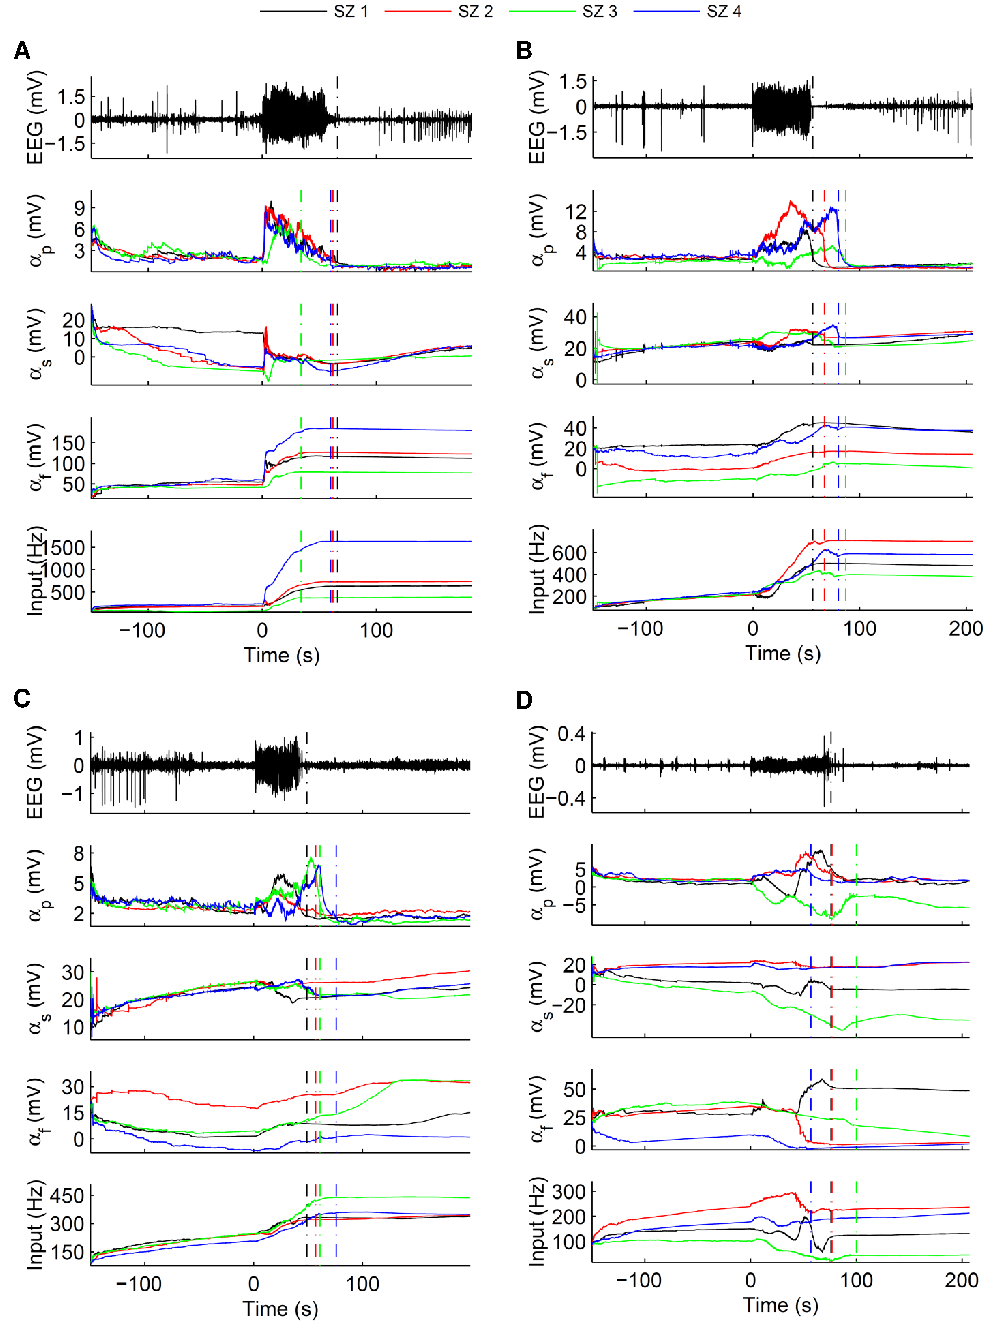
\includegraphics[max size={\textwidth}{\textheight}]{fig/EstimationFigures1.pdf}
 	\caption{Results from the estimation of four seizures from four different animals . (\textbf{A}), (\textbf{B}), (\textbf{C}), (\textbf{D}) Estimation results for four seizures(SZ) from animal 1-4, respectively. The colors in all graphs correspond to the legend above the figure. The first estimated seizure is shown in the top graph, where the initiation of seizure begins at time 0s and ends at the dotted black line. In the corresponding graphs the estimation results for the excitatory ($\alpha_{\mathrm{p}}$), slow inhibitory ($\alpha_{\mathrm{s}}$) and fast inhibitory ($\alpha_{\mathrm{f}}$) synaptic gains are demonstrated, where all seizures initiate at 0s and terminate at the dotted line with the same color. Lastly, the estimate for the mean input firing rate to the modeled population is demonstrated.}
 	\label{fig: EstimationResults}  
 \end{figure}

To validate the estimation results above we consider seizure one for each animal. Using the estimation results from seizure one we perform a forward simulation (Figure~\ref{fig: SZComp}). The results for seizure one from each animal are shown. It is clear from these figures that the estimation technique is capable of reproducing model parameters that are capable of producing simulated data similar to recorded EEG, in terms of the amplitude.  

\begin{figure}[ht]
 	\centering
 		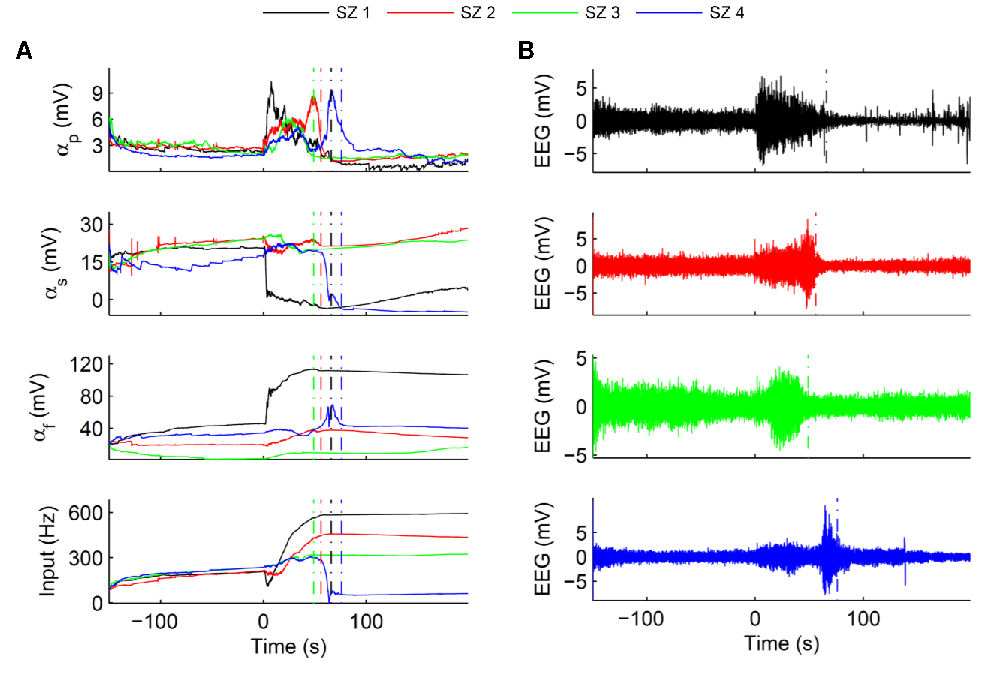
\includegraphics{fig/AnimalComp.pdf}
 	\caption{Estimation Results for Multiple Animals and Simulated EEG. (\textbf{A}) The results from seizures for four different animals. The estimated physiological parameters from each seizure (SZ) is specified by a different color line. All seizures initiate at time 0s and end at the dotted line that is the same color as the estimation results for the animal. (\textbf{B}) Artificial EEG generated using the neural mass model of the hippocampus. The artificial EEG is generated using the parameters from \textbf{A} with the same color as the traces in \textbf{B}.}
 	\label{fig: SZComp}
 \end{figure}

To demonstrate the robustness of the unscented Kalman filter to the starting values chosen for the estimation we have performed a monte carlo analysis~(Figure~\ref{fig: MonteResults}). In each trace the mean and covariance of the estimation over 100 simulations is shown. From these results it is clear that there is a higher level of variance on the fast synaptic inhibition ($\alpha_f$) and the input mean post seizure. However, the slow inhibitory gain standard deviation is higher preseizure. To compare the standard deviation over 100 estimations with the predicted error from the unscented Kalman filter we have plotted both results. The results show that there are similarities between the estimated error, and the error over multiple different intialised parameters. In particular, the estimation results preseizure for slow inhibition show a high standard deviation for both the single and monte carlo estimation procedure.

The results from figure~\ref{fig: MonteResults} also demonstrate the robustness of the unscented Kalman filter to the initialised parameters. In particular, when considering the mean over the monte carlo simulation and the results from a single estimation, there are clear similarities. The transition to and from seizure for all the model parameters have the same trends, and the standard deviation in both sets of results decreases during seizure periods. This may be due to a higher signal power in seizure periods. Another possible reason is that this model is created to represent both physiology, and seizure dynamics. Therefore, in seizure periods there is less uncertainty about the model predictions then there would be in background EEG.

The monte-carlo estimation also shows that there is a higher standard deviation post seizure compared to pre-seizure. This is due to the nature of the model, and the estimation results for the excitatory synpatic gain. Post seizure the excitatory synaptic gain is lower than any other period in the estimation procedure. When looking at the structure of the model, it is clear that when the excitatory synaptic gain is low the relative contribution of all other populations to the model output is low. With the correction step of the unscented Kalman filter the contribution of these populations would be seen to be similar to noise on the observations, therefore, there is higher uncertainty about these estimates. The reason for a high variance on the input is apparent, as it is the mean of a stochastic element. 

\begin{figure}[ht]
	\centering
		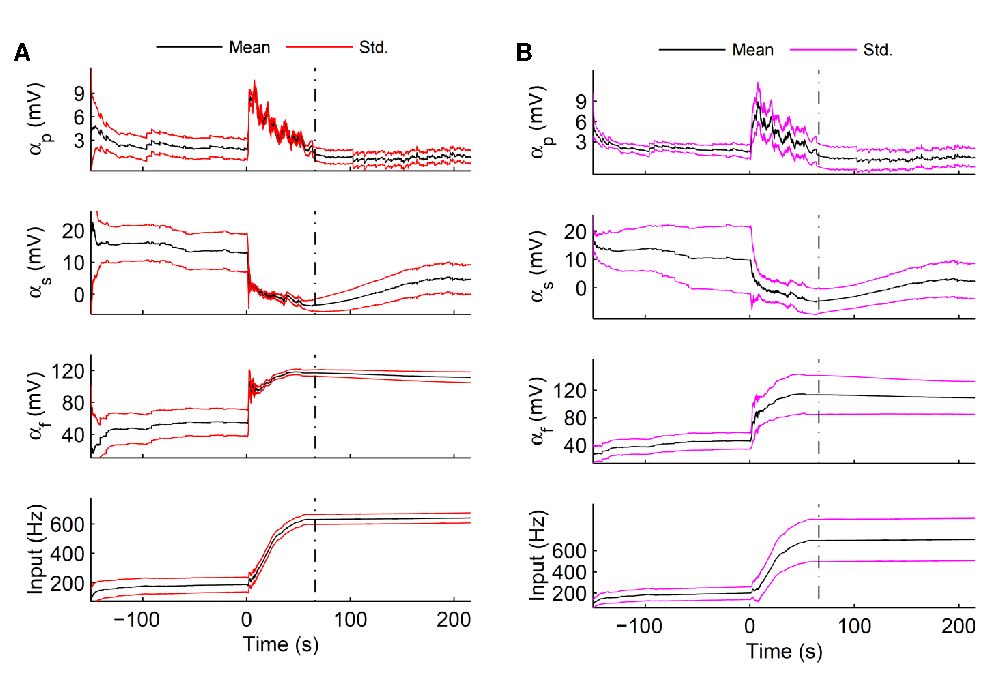
\includegraphics{fig/MonteResults.pdf}
	\caption{Comparison of the mean and standard deviation of a single and monte carlo analysis of the estimation technique. \textbf{A} Results from a single estimation are shown, where the standard deviation of each estimate made by the unscented Kalman filter is also shown in red. \textbf{B} The mean and standard deviation of 100 estimations using the same data set with different initial model parameters.}
	\label{fig: MonteResults}
\end{figure}
 